\documentclass{osa-article}
\usepackage{threeparttable}
\usepackage{lineno,hyperref}
\usepackage{indentfirst}
\usepackage[T1]{fontenc}
\usepackage{type1cm}
\usepackage{url} 
\usepackage{CJK}
\usepackage{xcolor,graphicx,float}
\usepackage{amsmath}
\usepackage{amssymb}
\usepackage{caption}
\usepackage{subcaption}
\usepackage{bm}
\usepackage{mathrsfs}
\modulolinenumbers[5]
\usepackage{color} % Allow text colors
%% Select the journal you're submitting to
%% oe, boe, ome, osac, osajournal
\journal{boe}
% Key:
% Express journals must have the correct journal selected:
% {oe} Optics Express
% {boe} Biomedical Optics Express
% {ome} Optical Material Express
% {osac} OSAC Continuum
% Other OSA journals may use:
% {osajournal} Applied Optics, Advances in Optics and Photonics, Journal of the Optical Society of America A/B, Optics Letters, Optica, Photonics Research

% Uncomment if submitting to Photonics Research.
% ONLY APPLICABLE FOR \journal{osajournal}
% \setprjcopyright

% Set the article type
\articletype{Research Article}
% Note that article type is not required for Express journals (OE, BOE, OME and OSAC)


\begin{document}

\title{Detection of Exudates in Fundus Photographs with Imbalanced Learning Using Conditional Generative Adversarial Network}


\author{Rui Zheng,\authormark{1,*} Lei Liu,\authormark{2,*}, Shulin Zhang,\authormark{1},Chun Zheng,\authormark{3},Filiz Bunyak,\authormark{4},Ronald Xu,\authormark{1}, Bin Li,\authormark{2}, Mingzhai Sun,\authormark{1} }


\address{\authormark{1}Department of Precision Machinery and Instrumentation, University of Science and Technology of China, Hefei, 230022, China\\
\authormark{2}Department of Electronic Engineering and Information Science, University of Science and Technology of China, Hefei, Anhui, 230022, China\\
\authormark{3}The 105 Hospital of PLA, Hefei, 230031, China\\
\authormark{4}The 105 Hospital of PLA, Hefei, 230031, China\\
}

\corresp{*These two authors contribute equally to the study. \\Corresponding author: Mingzhai Sun}
\email{mingzhai@ustc.edu.cn} %% email address is required

% \homepage{http:...} %% author's URL, if desired

%%%%%%%%%%%%%%%%%%% abstract %%%%%%%%%%%%%%%%
%% [use \begin{abstract*}...\end{abstract*} if exempt from copyright]

\begin{abstract}
Diabetic retinopathy (DR) is a leading cause of blindness worldwide. However, 90\% of DR caused blindness can be prevented if diagnosed and intervened early. Retinal exudates can be observed at the early stage of DR and could be used as signs for early DR diagnosis. Deep convolutional neural networks (CNNs) have been applied for exudate detection with promising results. However, there exist two main challenges when applying the supervised deep convolutional neural network based methods for exudate detection. One is the very limited number of labeled data available from medical experts, and another is the severely imbalanced distribution of data of different classes. First, there are much more images of normal eyes than those of eyes with exudates, particularly for screening datasets. Second, the normal pixels (non-exudates) are much more than the abnormal pixels (exudates) in images containing exudates. To tackle the small sample set problem, an ensemble convolutional neural network (MU-net) based on a U-net structure is presented in this paper. To alleviate the imbalance data problem, the conditional generative adversarial network (cGAN) is adopted to generate label-preserving minority class data specifically to implement the data augmentation.
Experiments on four representative public datasets show that our method outperformes not only the conventional state-of-the-art methods but also recent CNN based methods. CGAN, as an upsampling method, significantly improves network robustness and generalization properties.
\end{abstract}

\begin{keywords}
Diabetic retinopathy (DR), Exudates, Convolutional neural network (CNN), Conditional generative adversarial network (cGAN).
\end{keywords}


%%%%%%%%%%%%%%%%%%%%%%%%%%  body  %%%%%%%%%%%%%%%%%%%%%%%%%%
\section{Introduction}
\PARstart{A}{ccording} to 2016 WHO report, from 1980 to 2014 the number of adults living with diabetes has risen from 108 million to 422 million with the global prevalence increasing from 4.7\% to 8.5\%~\cite{mathers2006projections}. Among many complications that diabetes leads to, diabetic retinopathy (DR) is a significant cause of blindness. In 2010, DR caused 2.6\% of blindness~\cite{bourne2013causes}. DR occurs as a result of long-term accumulated damages to the small blood vessels in the retina. After 20 years of diabetes, nearly all patients with Type I diabetes and >60\% of patients with Type II diabetes have some degree of retinopathy~\cite{sirhindidiabetic}. At the early stage of DR, patients may not have any symptoms of vision problems. However, when it develops to the late stage, it may permanently cause vision loss and blindness. Therefore it is important for diabetic patients to have a comprehensive retina screening at least once a year. It is shown that blindness due to DR can be prevented in 90\% of the cases by early detection through regular screening~\cite{tapp2003prevalence}.

Fundus photography is the most commonly used and effective way of screening for diabetic retinopathy. Ophthalmologists look for early signs of DR such as exudates. Exudates are lipid and lipoprotein deposits that appear near leaking capillaries within the retina. They develop at the early stage of DR and may appear as yellow areas with variable sizes from a few pixels to as large as the optic disc (Fig.~\ref{fig:exudates}).

Fundus images are usually examined by ophthalmologists. However, due to the limited number of the eye doctors and the massive screening population, many computer-aided diagnosis systems (CAD) have been developed to automatically detect the typical pathological signs of DR in the hope of improving the screening efficiency and releasing the expensive medical resources. The sensitivity and accuracy of the CADs are critical for the early diagnosis. However, the low contrast, irregular shapes, and sparsity of the early signs of DR pose enormous challenges to the analysis methods.

\begin{figure}[ht]
\centering
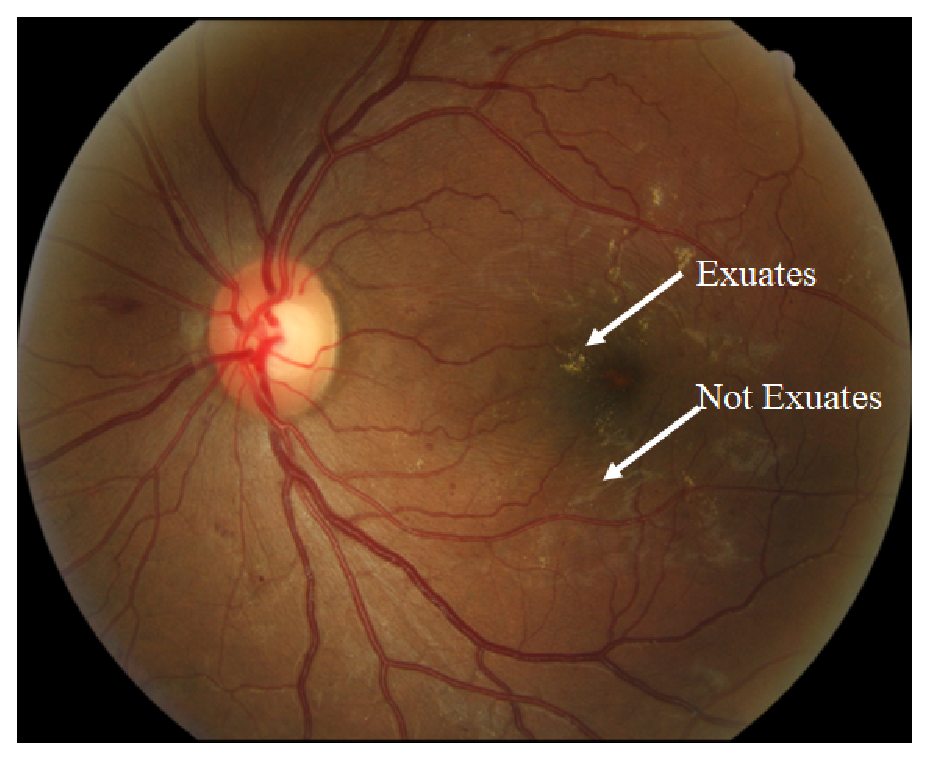
\includegraphics[width=0.8\linewidth]{display2.eps}
\caption{Retinal image with exudates.}
\label{fig:exudates}
\end{figure}

Deep convolutional neural networks have been proven to outperform conventional image analysis methods in many aspects, especially because they do not require explicit feature extraction. Recently, deep learning methods were applied to detect exudates in color fundus photographs and showed promising results although the highest reported sensitivity and accuracy were still lower than those using the state-of-the-art conventional image analysis methods~\cite{feng2017deep,pereira2015exudate, tan2017automated}. \textcolor{red}{The deep learning method in~\cite{feng2017deep} obtained a maximum sensitivity of 81.35\% while \cite{fraz2017multiscale} got an impressive sensitivity of 92.42\% on DIARETDB1 database in conventional image analysis methods.} The performance of the deep learning methods is mainly limited by two challenges. One is the limited expert labeled training data to train network, and the other is the severely imbalanced representations of different classes.

Limited expert-labeled data is a general problem in the medical image analysis field since it is usually costly to acquire the ground truth data. Imbalanced dataset manifests itself in two aspects. One is that there are much fewer images of pathological conditions than those of normal conditions. This is particularly true for datasets acquired during the massive screening, such as the DR screening. In these datasets majority of the images do not contain any pathological conditions. The other aspect of the imbalanced data is that the number of abnormal pixels is much less than that of the normal pixels. For example, in the image with only a few exudates, more than 98\% of the pixels are normal with about 2\% are abnormal pixels. This severely imbalanced representation of different classes renders great challenge for constructing a robust and reliable neural network with good generalization property.

To address the problems discussed hereinbefore, we developed an ensemble deep convolutional neural network (MU-net) based on the U-net framework that was mainly designed for medical applications with limited ground truth data. Furthermore, to solve the imbalanced class problem, we applied the conditional generative adversarial network (cGAN) to augment the dataset and specifically upsample the minority class. Our method significantly outperformed previous methods and had good generalization property over different datasets.


The paper is organized as follows. In section 2, we provide a short overview of different approaches used for exudate detection and discuss methods for imbalanced dataset learning. In section 3, we present detailed explanations of our approach. We illustrate the results in section 4 with discussions and end the paper in section 5 with a short conclusion. 


\section{Related works}
Automatic exudate detection in fundus images has been studied before, and many methods have been developed, including traditional image processing methods and recent approaches based on machine learning and neural networks. Thresholding methods based on global or local image gray-level~\cite{phillips1993automated,yazid2012automated,figueiredo2015automated,wisaeng2015automatic}, and clustering-based image thresholding, such as Otsu thresholding~\cite{yazid2012automated,wisaeng2015automatic}, have been applied for exudate segmentation. Methods based on morphological operations~\cite{walter2002contribution,sopharak2008automatic,welfer2010coarse,harangi2014automatic,imani2016novel,
fraz2017multiscale} have also been explored. In these methods, dominant structures, such as blood vessels and optic disc, were usually first identified and removed from the images to reduce the interference with the exudate segmentation. Region growing method~\cite{ege2000screening,sinthanayothin2002automated,li2004automated,usher2004automated} has also been demonstrated for automatic segmentation of exudates, particularly in combination with the artificial neural network~\cite{usher2004automated}.

Machine learning based methods, such as linear discriminant classifiers~\cite{sanchez2008novel,niemeijer2007automated}, support vector machine (SVM) ~\cite{fleming2007automated,giancardo2012exudate}, Naive Bayes classifier~\cite{harangi2012automatic} and random forest algorithm~\cite{zhang2014exudate}, have been studied. Most of these methods consisted of building a feature vector for each pixel or pixel cluster that was to be classified with a machine learning approach into exudates or non-exudates. The features were usually based on the color, brightness, size, shape, edge strength, texture, contextual information, etc. of the pixel clusters.

CNN has shown excellent performance in various applications including medical image processing. Pavle et al.~\cite{prentavsic2016detection} constructed a 10-layer of a neural network for exudates detection. In~\cite{feng2017deep}, Feng et al. applied a Fully Convolutional Neural Networks (FCN) to segment optic disc and exudates. Fujita et al.~\cite{tan2017automated} used a single convolutional neural network to detect exudates, hemorrhages, and microaneurysms simultaneously. CNN based methods demonstrated great promise in the fundus image analysis. However, compared to the conventional state-of-the-art methods, the performance of CNN based approach, particularly with the best-reported sensitivity of 87.58\%, still has much room for improvement. The weaker performance of the CNN based methods partially comes from the limited training data and the significantly imbalanced class data.

Imbalanced data poses enormous challenges to many classifiers, most of which are optimized to reduce global error rate without taking into consideration of data distribution. One straightforward method to alleviate the class imbalance problem is to upsample the minority class or to downsample the majority class. Synthetic minority over-sampling technique (SMOTE)~\cite{chawla2002smote} is an excellent method from this perspective. In this paper, we applied the cGAN framework to augment the training dataset and to upsample the minority class specifically. Our results demonstrated that this was an effective way to improve network robustness and generalization properties. 


\section{Proposed methodology}
In this section, we introduced the modified U-net (MU-Net) structure for exudate detection and demonstrated applying conditional generative adversarial network(cGAN) to generate synthetic images as a new method of data augmentation and minority class upsampling.

\subsection{Image pre-processing}
The images from different datasets were acquired with different types of fundus cameras, which rendered different image size, resolution and signal-to-noise ratio (SNR). To reduce the image variation from different datasets, we applied a pre-processing step before feeding the images to the neural network. First, all the images were resized to 580$\times$580 pixels. Second, only the green channels from the original RGB images were processed since the green channels showed the highest contrast of exudates from the background~\cite{gupta2016efficient}. Third, an adaptive contrast enhancement technique~\cite {sinthanayothin1999automated}  was applied to improve the contrast of exudates on the retinal surface.

\subsection{U-net and modified U-net (MU-net)}
U-Net was first proposed by Ronneberger \cite{ronneberger2015u} for biomedical image segmentation. It is a supervised method based on Convolutional Neural Networks (CNNs). It was designed to produce precise segmentation with a low number of training images, which was of particular importance for medical image applications since it was usually costly to label a large number of the medical images by medical experts. 

We constructed an U-net model with eleven convolutional layers (Fig.~\ref{fig:U-net}a). It had a downsampling and an upsampling paths. For each path, it consisted of three stacked convolution steps. In the downsampling path, two convolutional layers both with a 3$\times$3 kernel were followed by normalization and dropout. A leaky rectified linear unit (LeakyReLU) instead of a rectified linear unit (ReLU) as in the original study~\cite{ronneberger2015u}, was implemented as the activation function. LeakyReLUs allow a small, non-zero gradient when a unit is not active~\cite{maas2013rectifier}. A 2$\times$2 max pooling with a stride of two at each dimension was applied. In the upsampling path, similar to the downsampling path, two 3$\times$3 convolutional layers were followed by a LeakyReLU activation. An up-convolution with a kernel size of 2$\times$2 and stride of two in each dimension was applied and the output was fused with the corresponding layers in the downsampling path. In the last layer a 1$\times$1 convolution reduced the number of output channels to the number of labels, which was 2 in this case. The input of the network was 48$\times$48 image patches and the output image size was the same as the input.



\begin{figure*}[ht]
\centering
\includegraphics[width=1\linewidth]{3net.eps}
\caption{(a) Structure of the U-net; (b) A building block of the MU-net; (c) MU-net consisting of 4 building blocks with different filter sizes.}
\label{fig:U-net}
\end{figure*}


To improve the performance of the original U-Net, we constructed a modified U-Net (MU-Net)(Fig.~\ref{fig:U-net} a, b, c). The MU-net was an ensemble of four modified U-net building blocks (Fig.~\ref{fig:U-net}c). In the building block, the max pooling layer was rearranged to the deeper layer of the network. Max pooling layer is useful for dimension reduction and helps make the learned features more invariant to small translations of the input~\cite{bengio2015deep}, which is important for feature detection. However, positional information of a local maximum is lost after the max pooling operation. Such information is critical for accurate localization of the features. To preserve the position information, we applied the max pooling layer after the third convolution layer instead of the second one as in the original U-net.

Besides, MU-Net was an ensemble network. We applied the bootstrap aggregating (Bagging) method~\cite{breiman1996bagging} to improve the performance of the network in detecting exudates. Bagging is a powerful and reliable method for reducing generalization errors. Differences in model initialization or convolution kernel sizes, or selections of mini-batches are often enough to cause different members of the ensemble to make partially independent errors. As a result, neural networks usually benefit from model averaging even if all of the models are trained on the same dataset. In our case,  we constructed four models with the only difference in convolution kernel sizes (3$\times$3, 4$\times$4, 5$\times$5 and 6$\times$6). Convolutional layers with different kernel sizes have different receptive field and obtain different features. By averaging the four models, more detailed information was extracted and the network generalization error was reduced~\cite{lecun2015deep}.


\subsection{Conditional Generative Adversarial Network (cGAN) as a data augmentation and minority class oversampling method}

Over-fitting is a common problem for neural network models, especially for deep learning method that has a large number of parameters. In the medical image analysis, in addition to the constraint of the limited labeled data, extremely imbalanced class data renders another layer of difficulty. Imbalanced data has detrimental effects on the performance of classifiers usually by introducing significant biases and reducing the generalization property of the classifier. 

Data augmentation is an effective way to increase the size of the training dataset and reduces the degree of the over-fitting problem. By applying transformations, such as elastic distortion or affine transformation to the original data, data augmentation artificially increases the size of the training set~\cite{zhu2016adversarial}. However, conventional data augmentation methods do not solve the class imbalance problem. In the paper, we applied a cGAN framework not only for generating synthetic data but also as a method to upsample the minority class.

\begin{figure}[ht]
\centering
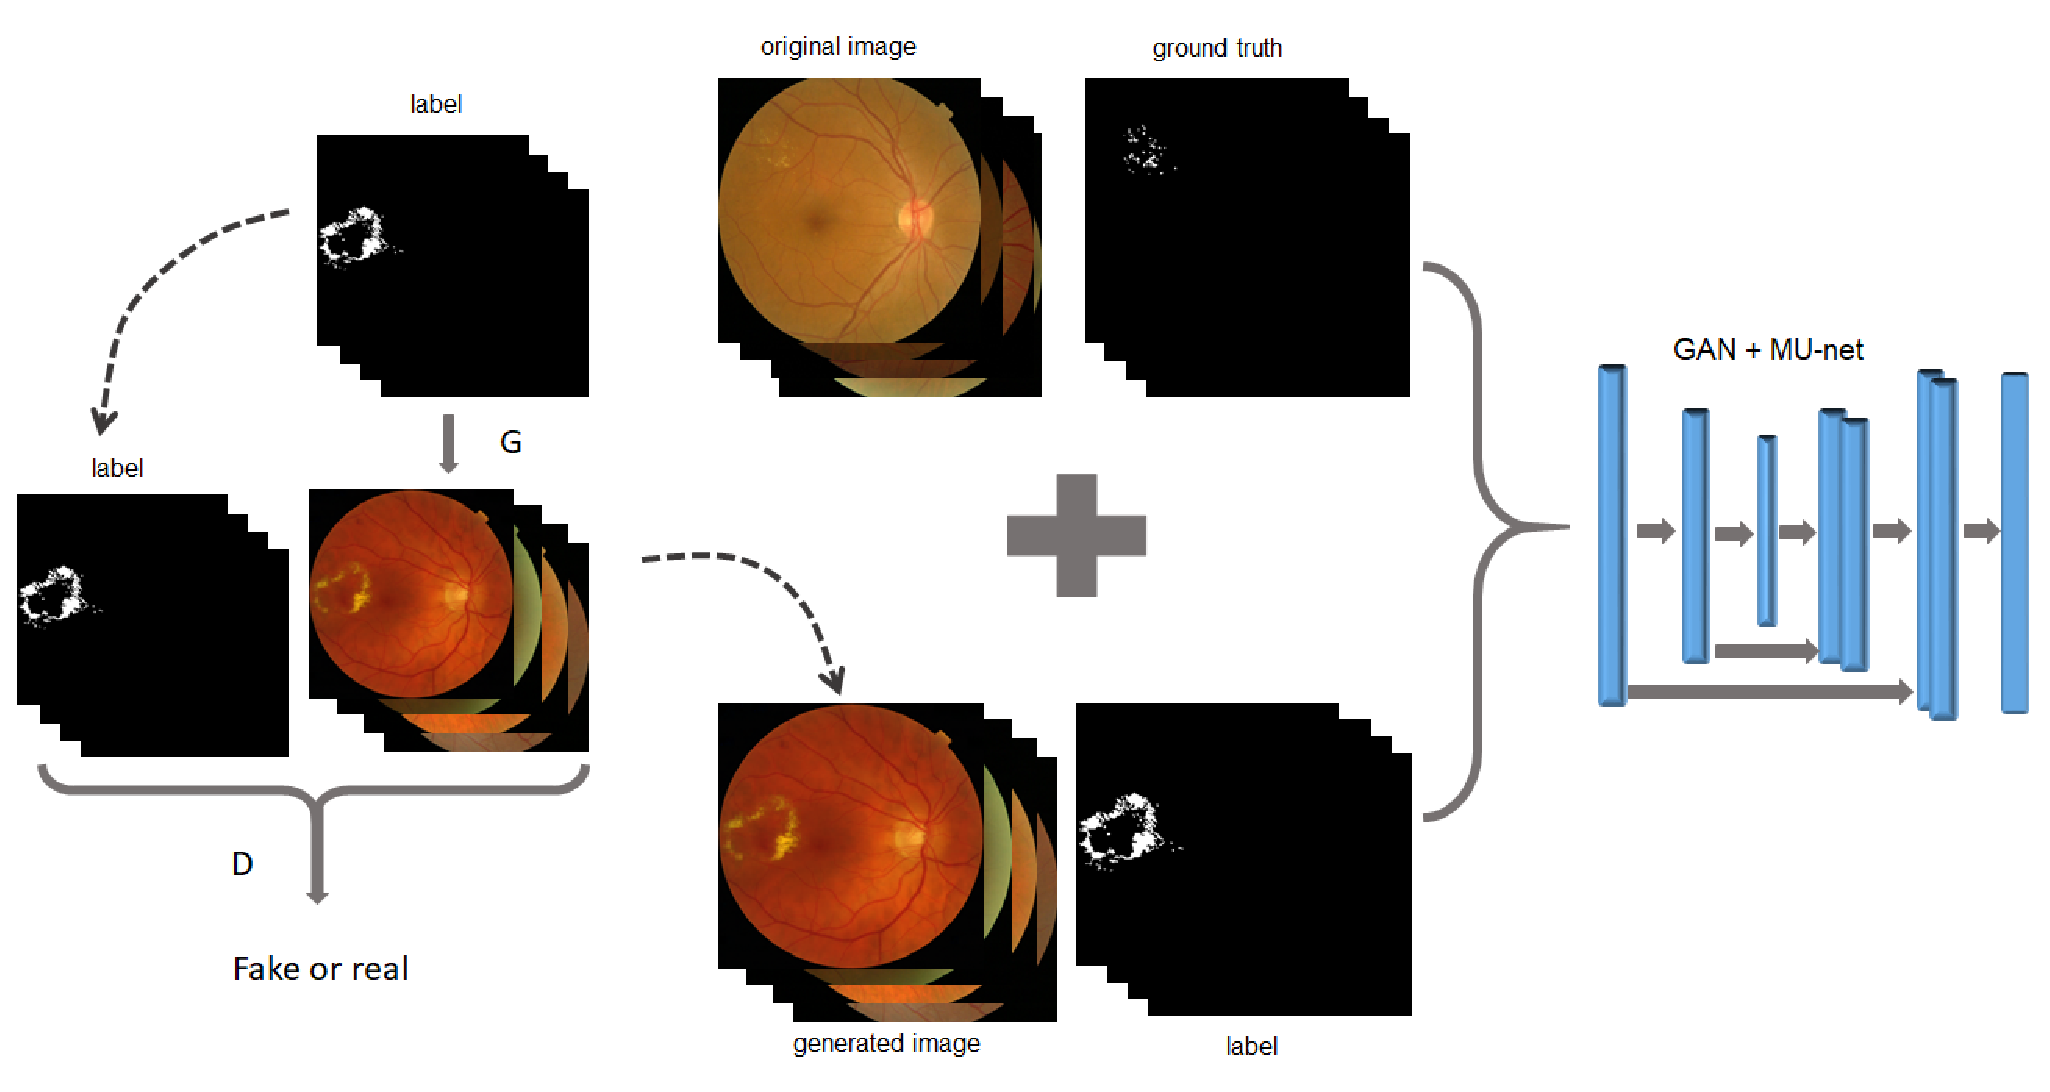
\includegraphics[width=0.95\linewidth]{structure.eps}
\caption{GAN+MU-net. The cGAN network was first trained to generate label preserving synthetic images (with details of the training process described in the main context). The synthetic image pair together with the real image pair from the training dataset were used to train the GAN+MU-net. }
\label{fig:net_structure}
\end{figure} 

\begin{equation}
G^* =arg\mathop{min}\limits_{G}   \mathop{max}\limits_{D}\mathcal{L}_{cGAN}(G,D) + \lambda \mathcal{L}_{L_1}(G)
\label{Eq:GAN_optimizer}
\end{equation}
GANs are generative adversarial networks proposed in~\cite{goodfellow2014generative,denton2015deep,radford2015unsupervised,salimans2016improved,isola2016image}. In the unconditioned GAN, the generator $G$ is trained to map from a random noise vector $z$ to the output vector $y: G:z \rightarrow y$ so that the synthetic vector $y$ is indistinguishable from the real vector as tested by an adversarially trained discriminator $D$. In conditional GANs (cGAN)~\cite{isola2016image}, besides the random noise vector $z$, an observed image $x$ is also supplied as the inputs. CGANs learn a mapping from the observed image $x$ and the random noise vector $z$, to $y: G:\{x, z\}\rightarrow y$ by optimizing the following objective:



where
\begin{equation}\label{eqn3_2}
\begin{aligned}
\mathcal{L}_{cGAN}(G,D) =& \mathbb{E}_{(x,y)\sim p_{data}(x,y)}[log{D(x,y)}]\\& + 
\mathbb{E}_{x\sim P_{data}(x), z\sim p_z(z)}[log(1 - D(x, G(x, z)))]\\
\end{aligned}
\end{equation}

\begin{equation}
\mathcal{L}_{L_1}(G) = \mathbb{E}_{(x,y)\sim p_{data}(x,y),(z)\sim p_z(z)}[\|y -G(x,z)\|_1] 
\label{Eq:cGAN_obj}
\end{equation}

We adapted the cGAN architecture from pix2pix in~\cite{isola2016image}. Two key features of the pix2pix framework were U-Net \cite{ronneberger2015u} based generator and a Markovian discriminator (PatchGAN). The U-Net based generator allowed low-level image information to shortcut across the network to achieve more realistic images. \textcolor{red}{In our experiments, $x$ was exudates groundtruth image input, $z$ was noise and $y$ was the corresponding RGB image output. }


\subsection{Evaluation metrics}
We evaluated the performance of the proposed methods based on both lesion level~\cite{wolf2006object} and image level measurements. For the lesion level evaluation, we compared the predicted candidates with the truly labeled exudates provided in the datasets. Instead of directly counting the number of pixels that were correctly classified or misclassified, we applied the approach based on set operations~\cite{zhang2014exudate, wolf2006object}. Briefly, if the two sets had enough overlap as controlled by an overlapping factor $\sigma$, which was set to 0.2 in our study, the same as in~\cite{zhang2014exudate}, the candidates were considered correctly classified. We computed the sensitivity, precision and the F1-score according to the equations defined in Table.~\ref{table:evaluation_metric}.
\begin{table}[htbp]
\centering
\begin{threeparttable}
\centering
\caption{Definitions of the evaluation metrics}
\begin{tabular}{ll}
\hline
 Performance Measure & Mathematical Formula \\
\hline
Accuracy & (TP+TN)/(TP+TN+FN+FP) \\
Sensitivity & TP/(FN+TP) \\
Specificity& TN/(FP+TN)  \\
Precision & TP/(FP+TP)  \\
F1-Score & 2*TP/(2*TP+FP+FN)\\
\hline
\end{tabular}
\label{table:evaluation_metric}
\begin{tablenotes}
\item[1] TP stands for true positive. FP: false positve; TN:  true negtive; FN: false negative.
\end{tablenotes}
\end{threeparttable}
\end{table}

For the image level evaluation, \textcolor{red}{full image consisting of exudates was regarded as correctly classified if the program detected right exudate candidate.}  A false positive image was defined as an image that had no exudates, but the program falsely detected some candidates. A false negative image was an image that had exudates, but the program did not detect any candidate. A true positive or a true negative image was defined as an image with or without any exudates and was correctly classified by the program. 


\section{Experimental results and discussion}
\subsection{Datasets} 
We used four public datasets in the study: e\_ophtha\_EX \cite{zhang2014exudate}, DIARETDB1 \cite{kauppi2007diaretdb1}, HEI-MED~\cite{giancardo2012exudate} and MESSIDOR \cite{decenciere2014feedback}. However, training of the networks was done only with the e\_ophtha\_EX dataset, while the other three were used to test the performance of the networks. 


The e\_ophtha\_EX dataset consists of 82 fundus images with four different image sizes of 1440$\times$960 or 1504$\times$1000 or 2544$\times$1696 or 2048$\times$1360 pixels. All images were acquired with a 45-degree field of view. Forty-seven of the images have exudates that were carefully marked by two ophthalmologists. The other
35 images do not contain exudates. 


The DIARETDB1 dataset contains 89 images with an image size of 1500$\times$1152 pixels. All the images were captured using the same 50-degree field-of-view digital fundus camera with varying imaging settings. Eighty-four images in the dataset contain at least mild non-proliferative signs, such as microaneurysms, of the diabetic retinopathy, and 5 images are considered as normal. 

The HEI-MED dataset consists of 169 fundus images that are representative of a various degree of diabetic macular edema (DME) with a resolution of 2196$\times$1958 pixels and with a 45 Field of View (FOV). All the images were captured with a Zeiss Visucam PRO fundus camera. 115 images are considered as normal retinal images and 54 retinal images are diagnosed with diabetic macular edema.

The MESSIDOR dataset is the largest fundus image database, which contains 1200 TIFF images with three different image sizes, 1440$\times$960, 2240$\times$1488 and 2304$\times$1536 pixels. All the images were acquired using a color video 3CDD camera on a TopCon TRC NW6 with a 45-degree field of view. 800 images were acquired with pupil dilation and 400 without dilation. However, the MESSIDOR dataset does not have the ground truth of the exudates. To perform the detailed evaluation of the proposed system for exudate detection, we manually annotated the exudate pixels of 80 images with the help of two ophthalmologists.  Labels at the image level, i.e., whether an image containing exudate or not, were generated for all the 1200 images. Our manually annotated dataset is available upon request.


\subsection{Training and testing of the networks}
It is worth to note that training of the networks was done only with the e\_ophtha\_EX dataset. All the other three datasets were used as testing datasets to evaluate the network performance only.

In the e\_ophtha\_EX dataset, there are 82 labeled images of which 47 images consisting of exudates. During the training phase, 60 images (35 with and 25 without exudates) were used as the training images, and the other 22 images (12 with and 10 without exudates) were used as the testing images. 


We adapted the cGAN architecture from pix2pix in~\cite{isola2016image}. During the training phase, the input of the pix2pix network was an image pair of the original RGB image with the corresponding binary ground truth image from the training set in e\_ophtha\_EX. All the weights were initialized from a gaussian distribution with mean 0 and standard deviation 0.02. To optimize the network, we alternated between one gradient descent step on the discriminator $D$, then one step on the generator $G$~\cite{isola2016image}. We applied the Adam solver~\cite{kinga2015method}, with learning rate of 0.0002, and the momentum parameters $\beta_1=0.5, \beta_2=0.999$.  The pix2pix network was trained for 350 epochs with batch size of 1. During the image generation phase, the input of the pix2pix network was a binary ground truth image from the training set, and the output was a synthetic image that was similar to but different from the input of the network. We applied the trained pix2pix network to all the 60 binary ground truth images to generate 60 synthetic images. Then we train the pix2pix for a second time independently without using the first trained weights. After that, with the second time trained pix2pix we generate another 60 synthetic images. \textcolor{red}{ Majority of the synthetic images were very similar to the real images in the sense of general looking and appearance of exudates, but some with obvious artifacts as shown in Fig.~\ref{fig:GAN-generated}. In total, 120 synthetic images were generated, among which 86 images with no or small artifacts were selected.  } 

\begin{figure*}[ht]
\centering
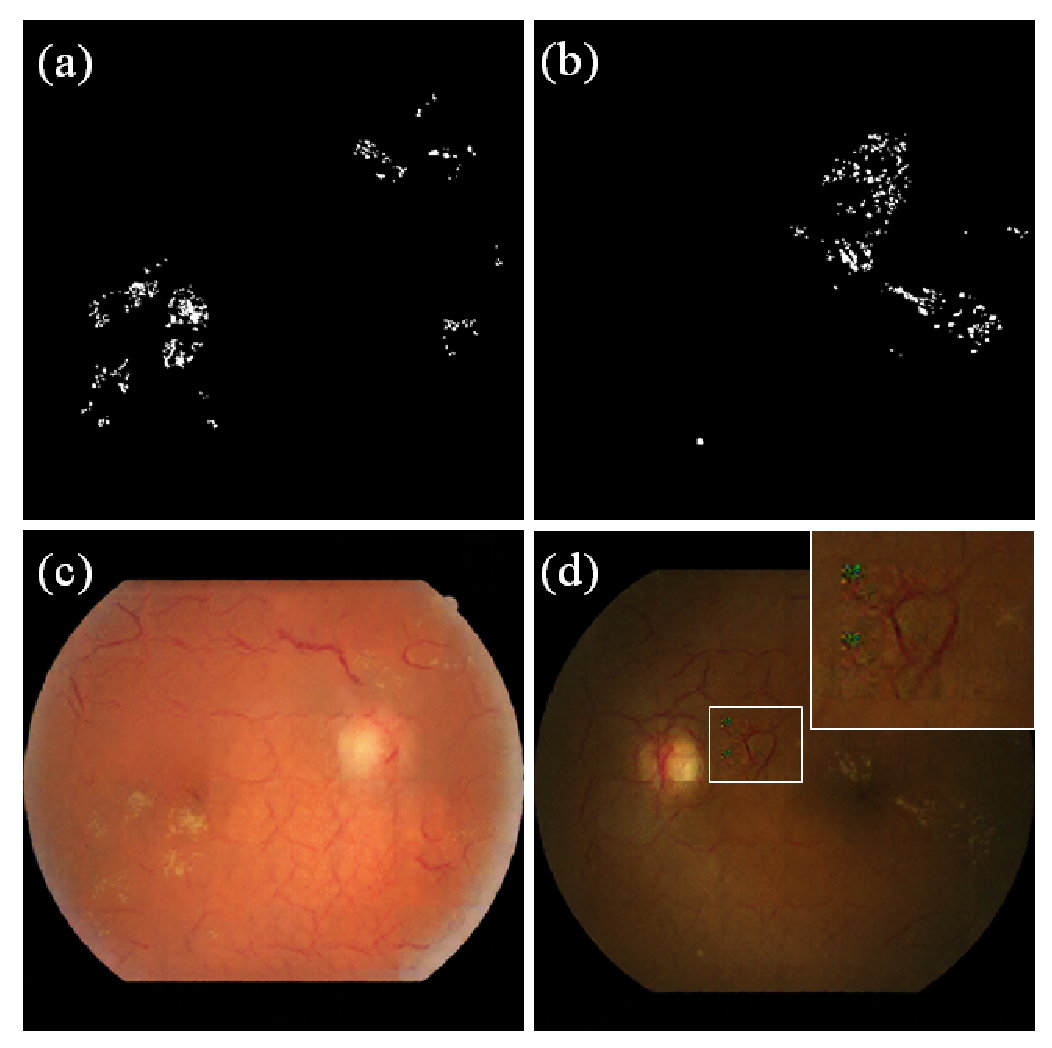
\includegraphics[scale=0.6]{GAN_img.eps}
\caption{Synthetic images generated using cGAN. (a) and (b) were the labeled binary images with the corresponding synthetic images (c) and (d) respectively.  (c) was a good synthetic image without any noticeable artifacts, while (d) showed some artifacts. The inset in (d) was the enlarged version of the white rectangle area.  }
\label{fig:GAN-generated}
\end{figure*}


To fully utilize the limited data, we applied a patch-based training process. We partitioned the image pair (the original RGB image and the corresponding ground truth image) into 48$\times$48 patches. 
We used two different partitioning approaches: selective partitioning and uniform partitioning, and we named the generated patches as "selective patches" and "uniform patches". For the selective partitioning, we randomly selected a pixel from the set of the exudate pixels of an image. With the selected exudate pixel $(x_i, y_i)$ as the reference point, we got a 48$\times$48 block of the image {\{($x_{i-23}$, $y_{i-23}$), ($x_{i-22}$, $y_{i-22}$), ..., ($x_{i+25}$, $y_{i+25}$)\}}. This approach ensured that the selected patch contained contain exudate pixels. Patches selected this way may overlap. Similarly, to do the uniform partition, \textcolor{red}{All images were uniformly cut into 48$\times$48 patches, and the patches were also overlapped. Since there was only a small percentage of the image pixels were exudate pixels, the majority of the uniform patches did not consist of exudate pixels.} 

We applied a two-stage training process for the U-net, MU-net, \textcolor{red}{MU-net block} and the GAN+MU-net.  

For the U-net, \textcolor{red}{MU-net block} and the MU-net, at the first stage, 67,200 patches were used to train the networks. 75\% of these patches (50,400 patches) were selective patches(with exudates), and 25\% of them were uniform patches(without exudates). We experimented the ratio between the selective and the uniform patches and empirically found this one rendered the best results. Obviously, at this stage, the minority class (exudate pixel) was upsampled to alleviate the imbalanced data problem. At the second stage, 47,040 uniform patches were generated and used to fine tune the network. The purpose of the second stage training was to enhance the diversity of the samples and to reduce the false positive detections. 



For the GAN+MU-net, besides the 60 training images from the e\_ophtha\_EX dataset, we generated 86 synthetic
images using the trained pix2pix network as described previously. 81,760 selective and 114,464 uniform patches were applied at the first and the second stage training, respectively.

For all the training at both stages, we applied stochastic gradient descent with a batch size of 64, a momentum of 0.3, and weight decay of $10^{-6}$. We initialized the weights in each layer from a zero-mean gaussian distribution with a standard deviation of 0.01. The learning rate was initialized to 0.01. Dropout was applied to alleviate overfitting, and the rate was set to 0.2. We trained 400 epochs at the first stage and fine-tuned the networks at the second stage for another 400 epochs.

All the trained networks were tested using the left 22 images in the e\_ophtha\_EX  dataset to evaluate the performance. Besides, MU-net and GAN+MU-net were further tested on the other three datasets (DIARETDB1, HEI-MED, and MESSIDOR) to assess the generalization property of the networks.



\subsection{MU-net significantly improved exudate segmentation}

Compared with the original U-net, \textcolor{red}{our MU-net block clearly outperformed the original U-net by a much large margin as tested both on the lesion level and image level(Table~\ref{tab:performance of U-net models on lesion level} and \ref{tab:performance of U-net models in image level}). F-1 score of MU-net was 1\% higher than MU-net block, it showed that the combination of four U-net can also improve performance of network.}  The sensitivity of MU-net was more than 10\% higher than that of the original U-net, and the precision and F-1 score were more than 8\% higher. On the image level, the accuracy of MU-net was 22.75\% higher than the original U-net. 

\begin{table}[htbp]
\centering
\begin{threeparttable}
\small
\setlength\tabcolsep{10pt}
\caption{Evaluation of the performance of U-net, \textcolor{red}{MU-net block,} MU-net and GAN+MU-net at the lesion level. It was evaluated using the 22 test images (12 images with and 10 without exudates) in the e\_ophtha\_EX dataset.} 
\begin{tabular}{lcccccc}
\hline
 & Accuracy & Specificity & Sensitivity & Precision & F1-score \\
\hline
U-net & $99.94\%$ & $99.97\%$ & $83.49\%$ & $85.16\%$ & $84.32\%$ \\
MU-net block & $99.95\%$ & $99.97\%$ & $\bm{92.60\%}$ & $89.67\%$ & $91.11\%$ \\
MU-net & $99.96\%$ & $99.98\%$ & $\bm{94.12\%}$ & $91.25\%$ & $92.66\%$ \\
GAN+MU-net & $\bm{99.97\%}$ & $\bm{99.99\%}$ & $90.94\%$ & $\bm{94.72\%}$ & $\bm{92.79\%}$ \\
\hline
\end{tabular}
\label{tab:performance of U-net models on lesion level}
\end{threeparttable}
\end{table}

\begin{table}[htbp]
\centering
\begin{threeparttable}
\small
\setlength\tabcolsep{28pt}
\caption{Evaluation of the performance of the U-net, \textcolor{red}{MU-net block}, MU-net and GAN+MU-net at the image level using the 22 test images in the e\_ophtha\_EX dataset.} 
\begin{tabular}{lccc}
\hline
 & True & False & Accuracy \\
\hline
U-net & $14$ & $8$ & $63.64\%$ \\
MU-net block & $17$ & $5$ & $77.27\%$ \\
MU-net & $19$ & $3$ & $86.39\%$ \\
GAN+MU-net & $21$ & $1$ & \bm{$95.45\%}$ \\
\hline
\end{tabular}
\label{tab:performance of U-net models in image level}
\end{threeparttable}
\end{table}

\begin{figure}[ht]
\centering
\includegraphics[width=\linewidth]{4net_ROC_PR.eps}
\caption{(a) ROC curves of the U-net, MU-net block, MU-net and GAN+MU-net. (b) Precision-Recall curves of the four networks. GAN+MU-net had the highest AUCs as calculated either with the ROC curves or the Precision-Recall curves.}
\label{fig:4net_PR_POC}
\end{figure}

Fig.~\ref{fig:4net_PR_POC} showed the ROC and the Precision-Recall(P-R) curves with the AUCs of the U-net, MU-net block, and MU-net. \textcolor{red}{The AUCs of the MU-net block calculated both using the ROC and the P-R curves were higher than those of the U-net. The AUCs of the MU-net were also higher than MU-net block, it showed that four networks  combined can help improve performance of network.} The curves of the MU-net completely enclose of the U-net, demonstrating that the MU-net outperforms the U-net by a large margin. 


\subsection{cGAN improved the performance of MU-net in exudate segmentation}
 
To further resolve the imbalanced data problem, we applied the cGAN framework to generate synthetic images consisting of exudates. In Fig.~\ref{fig:GAN-generated}, the first row showed the ground truth binary images from the training dataset and the second row showed the generated synthetic images using the cGAN method. Majority of the generated images consist of very realistic exudates (Fig.~\ref{fig:GAN-generated}(c)), but some generated exudates showed artifacts (Fig.~\ref{fig:GAN-generated}(d)). This is consistent with previous studies that some GAN generated images are far from realistic images, which was noted before and thought as a general problem of GAN~\cite{isola2016image}. The synthetic images together with the true images from the training dataset(Fig.~\ref{fig:net_structure}) were used to train the MU-net, which we named it as GAN+MU-net. 

\begin{table}[htbp]
\centering
\caption{Comparison of the performances at the lesion level of the MU-net and GAN+MU-net using different testing datasets to test the generalization property of the networks.} 
\begin{tabular}{llccccc}
\hline
Database & Methodology &  Accuracy & Specificity & Sensitivity & Precision & F1-Score  \\
\hline
e\_ophtha\_EX & MU-net & $99.96\%$ & $99.98\%$ & $\bm{94.12\%}$ & $92.15\%$ & $92.66\%$\\
        & GAN+MU-net & $\bm{99.97\%}$ & $\bm{99.99\%}$ & $90.94\%$ & $\bm{94.72\%}$ & $\bm{92.79\%}$ \\
\hline
DiaRetDB1 & MU-net & $99.96\%$ & $99.98\%$ & $91.72\%$ & $\bm{91.10\%}$ & $91.41\%$ \\
        & GAN+MU-net & $\bm{99.97\%}$ & $99.98\%$ & $\bm{93.94\%}$ & $91.02\%$ & $\bm{92.46\%}$ \\
\hline
HEI-MED & MU-net & $99.94\%$ & $99.97\%$ & $91.02\%$ & $90.39\%$ & $90.72\%$ \\
       & GAN+MU-net & $\bm{99.95\%}$ & $\bm{99.98\%}$ & $\bm{90.67\%}$ & $\bm{91.88\%}$ & $\bm{91.27\%}$\\
\hline
MESSIDOR & MU-net & $99.95\%$ & $99.97\%$ & $91.46\%$ & $89.72\%$ & $90.58\%$ \\
        & GAN+MU-net & $\bm {99.96\%}$ & $\bm{99.99\%}$ & $\bm{95.33\%}$ & $\bm{93.38\%}$ & $\bm{94.34\%}$ \\
\hline
\end{tabular}
\label{tab:comparison of performances on different training set on pixel level}
\end{table}



Table~\ref{tab:performance of U-net models on lesion level} showed the comparison of MU-net and GAN+MU-net. Both the precision and F-1 score were significantly increased in GAN+MU-net though the sensitivity of GAN+MU-net decreased. However, on the image level, GAN+MU-net performed significantly better than MU-net with more than 9.06\% of increase of the accuracy (Table~\ref{tab:performance of U-net models in image level}). The AUCs of the GAN+MU-net were also higher than those of the MU-net (Fig.~\ref{fig:4net_PR_POC}).
\begin{table}[H]
\centering
\caption{Comparison of the performances of MU-net and GAN+MU-net on different testing datasets evaluated at the image level.} 
\small
\setlength\tabcolsep{20pt}
\begin{tabular}{llccc}
\hline
 Database & Network & True & False & Accuracy \\
\hline
e\_ophtha\_EX & MU-net & $19$ & $3$ & $86.39\%$ \\
           & GAN+MU-net & $21$ & $1$ & $\bm{95.45\%}$ \\
\hline
DiaRetDB1 & MU-net & $78$ & $11$ & $87.64\%$  \\
         & GAN+MU-net & $82$ & $7$ & $\bm{92.13\%}$ \\
\hline
HEI-MED & MU-net & $129$ & $40$ & $76.33\%$  \\
      & GAN+MU-net & $150$ & $19$ & $\bm{88.76\%}$ \\
\hline
MESSIDOR & MU-net & $1037$ & $163$ & $86.42\%$ \\
        & GAN+MU-net & $1075$ & $125$ & $\bm{89.58\%}$ \\
\hline
\end{tabular}
\label{tab:comparison of performances on different training Set on image level}
\end{table}


\subsection{cGAN improved the generalization property of the MU-net}
\begin{table}[htpb]
\centering
\small
\setlength\tabcolsep{12pt}
\caption{Comparison of the performances of our method with previous published methods using the four public datasets} 
\begin{tabular}{llcccc}
\hline
Database & Methodology &  Accuracy & Specifity & Sensitivity & Precision  \\
\hline
e\_ophtha\_EX & Moazam {et al.}\cite{fraz2017multiscale} & $89.25\%$ & $94.60\%$ & $81.20\%$ & $90.91\%$ \\
            & Zhang {et al.}\cite{zhang2014exudate} & $--$ & $--$ & $74\%$ & $79\%$  \\
            & Proposed & $\bm{99.97\%}$ & $\bm{99.99\%}$ & $\bm{90.94\%}$ & $\bm{94.72\%}$ \\
\hline
DiaRetDB1 & Moazam {et al.}\cite{fraz2017multiscale} & $87.72\%$ & $81.25\%$ & $92.42\%$ & $87.14\%$ \\
         & Rajan {et al.}\cite{rajan2016analytical} & $85.39\%$ & $85\%$ & $86.2\%$ & $--$  \\
         & Araujo {et al.}\cite{araujo2013automatic}& $99.25\%$ & $99.44\%$ & $80.83\%$ & $15.57\%$  \\
        & Proposed & $\bm{99.97\%}$ & $\bm{99.98\%}$ & $\bm{93.94\%}$ & $\bm{91.02\%}$  \\
\hline
HEI-MED & Moazam {et al.}\cite{fraz2017multiscale} & $95.77\%$ & $96.41\%$ & $\bm{94.63\%}$ & $\bm{93.72\%}$ \\
      & Akram {et al.}\cite{akram2014automated} & $92.5\%$ & $94.7\%$ & $96.1\%$ & $--$ \\
      & Ali {et al.}\cite{ali2013statistical} & $--$ & $--$ & $--$ & $82.6\%$  \\
      & Proposed & $\bm{99.95\%}$ & $\bm{99.98\%}$ & $90.67\%$ & $91.88\%$ \\
\hline
MESSIDOR & Agurto\cite{agurto2014multiscale} & $85.2\%$ & $90.2\%$ & $80.9\%$ & $--$ \\
         & Moazam {et al.}\cite{fraz2017multiscale} & $98.36\%$ & $96.41\%$ & $94.63\%$ & $92.72\%$ \\
         & Proposed & $\bm{99.96\%}$ & $\bm{99.99\%}$ & $\bm{95.33\%}$ & $\bm{93.38\%}$ \\
\hline
\end{tabular}
\label{tab:comparison_others}
\end{table}                                                              
Generalization property is an important measure of the performance of a network. It reflects how well the trained network can be applied to similar but different datasets. We applied the trained MU-net and GAN+MU-net on the other three public datasets. 

Table ~\ref{tab:comparison of performances on different training set on pixel level} and table ~\ref{tab:comparison of performances on different training Set on image level} showed the comparison results of MU-net and GAN+MU-net as evaluated using lesion level and image level measurements. In general, GAN+MU-net method outperformed MU-net in segmenting exudates. Specifically, GAN+MU-net achieved segmentation accuracy on image level of 92.13\% on Diaretdb1 dataset, 88.76\% on HEI-MED dataset, and 89.58\% on the MESSIDOR dataset, which were more than 4\%, 12\%, and 3\% higher than that of the MU-net, respectively. On the lesion level, GAN+MU-net also showed improved performance, especially as measured by the more comprehensive F1-score. It is conclusive that GAN+MU-net has better generalization property than MU-net. 
 

\subsection{Comparison with previous studies}
We compared our results with recent published literatures on exudate detection (Table~\ref{tab:comparison_others}). In the study we tested our method using four public datasets. Some of the listed methods in table ~\ref{tab:comparison_others} only applied on one of the datasets and not all the evaluation metrics were calculated. 
All the listed studies applied the same lesion level evaluation~\cite{wolf2006object} method as in our study. 
From the table, it was clear that our proposed GAN+MU-net surpassed most of the methods except the one proposed by Moazam {et al.}~\cite{fraz2017multiscale} on the HEI-MED dataset, although on all the other three datasets our method showed better performance than theirs. First, the color of the images in HEI-MED was much different from the e\_ophtha\_EX dataset, which may deteriorate the performance of the network that was trained on the e\_ophtha\_EX dataset. Second, in~\cite{fraz2017multiscale}, the authors trained the network using the HEI-MED dataset and tested the performance on the same dataset, which usually gave better performance. \textcolor{red}{Because the MESSIDOR dataset didn't have public exudates label, we are unable to replicate other performance measure because the ground truths they have used are not available online. we manually annotated the exudate pixels of 80 images (40 with exudates and 40 without exudates) with the help of two ophthalmologists. From the table, it can be clearly seen that our algorithm worked well on exudates segmentation.}
                     

\section{Conclusion}
Detection of exudates is important in preventing DR caused blindness. In the study we sought to develop a deep convolutional neural network based method for automatic exudate detection. In order to alleviate the two challenges -- limited expert labeled training data and imbalanced class data -- we developed an ensemble MU-net and a cGAN based data augmentation and minority class oversampling method. Training of the network with cGAN generated synthetic images significantly improved network performance, particularly its generalization property across different datasets. As we have been writing the paper, we note that recent study by Douzas~\cite{Douzas:2018ka} came to the same conclusion, demonstrating that conditional generative adversarial networks could be an effective data generation method for imbalanced learning.

\bibliography{mybibfile}


\end{document}


